\documentclass{school-22.101-notes}
\date{December 15, 2011}

\begin{document}
\maketitle


%% Part 2: Angular Momentum, Deuteron, 

\clearpage
\topic{Angular Momentum} 
  \begin{enumerate}
  \item Most basic properties about angular momentum:
    \eqn{ [V_i, J_j] &= i \hbar \epsilon_{ijk} V_k}
    which leads to: $[L_x, L_y] = i \hbar L_z, [L_y, L_z] = i \hbar L_x, [L_z, L_x] = i \hbar L_y$. 
    \eqn{[J^2, \vecn \cdot J] &= 0}

  \item Raising and lowering operators satisfy,
    \eqn{ J_+ &= J_x + i J_y & J_- &= J_x - i J_y }
    \eqn{ [J_z, J_-] &= - \hbar J_-   &J_- \ket{z} &= \alpha \ket{z-1} }

  \item $L, S, J$ all share the following: where $\ket{jm} = Y_l^m (\theta, \psi)$; remember that we can only do this for symmetric $V(r)$ such that we can write $\psi = R(r) \psi_l^m (\theta, \phi)$. 
    \eqn{ J^2 \ket{jm} &= j (j+1) \hbar^2 \ket{j m }    & J_z \ket{jm} &= m \hbar \ket{j m} }
    \eqn{ J_{\pm} \ket{jm} &= \hbar \sqrt{j(j+1) - m(m\pm 1)} \ket{jm \pm 1}  }
    \eqn{ J_x \ket{jm} &= \frac{\hbar}{2} (\sqrt{j(j+1) - m(m+1)} \ket{jm+1} + \sqrt{j(j+1) - m(m-1)} \ket{jm-1})  }
    \eqn{J_y \ket{jm} &= \frac{\hbar}{2} (-\sqrt{j(j+1) - m(m+1)} \ket{jm+1} + \sqrt{j(j+1) - m(m-1)} \ket{jm-1})  }    

\item The difference b/w $L$ and $J$:  
  \begin{enumerate}
  \item $l$ (orbital): integers, $0 \le l \le n$. A subset of $j$ is the solution from orbital component. 
  \item $j$ (total): integer steps, $|l-s|, \cdots, |l+s|$. It completely construct $l$ and $s$. 
  \item $m_j$ (z-component of total): $-j, \cdots j$ (includes 0 when $j$ is an integer, and does not include 0 when $j$ is a half-integer). Its degeneracy is $2j+1$. 
  \end{enumerate}



\item Angular momemtum addition: given any two of $s, l, j$ (or given $l_1, l_2$ and solving for total $l$), we can compute the 3rd one by taking integer steps from the difference to the maximum. Example: 
  \eqn{ |s-l| &\le j \le s+l   & |s-j| &\le l \le s+j }


\item Degeneracy: if we add two particles, the total degeneracy is: $2(2l_1+1) \times 2(2l_2 +1)$ where the $2$ comes from spin. 
  \end{enumerate}




\clearpage
\topic{Deuteron}
\textbf{Radial Schroedinger Equation:} Hamiltonian in general is, 
\eqn{ H = KE + PE = \frac{p^2}{2m} + V(r) = - \frac{\hbar^2}{2m} \laplacian + V(r) }
When we have to deal with two particles, we pick CM system, so $H = H_{CM} + H_{rel} = H_{rel}$, and we further expand $H_{rel}$ into the linear momentum part and the angular momentum part (by writing $\laplacian$ out in $r,\theta, \phi$ terms; a simple way to remember is, because $L = p r$, so ): 
\eqn{ H = H_{rel} = - \frac{\hbar^2}{2\mu} \frac{1}{r^2} \ddr \left( r \ddr \right) - \frac{L^2}{2 \mu r^2} = - \frac{\hbar^2}{2\mu} \frac{1}{r^2} \ddr \left( r \ddr \right) - \frac{\hbar^2 l (l+1)}{2 \mu r^2} }
Basically in one particle space, there is only linear KE; now there is angular KE, we combine it with the potential to define an effective potential: 
\eqn{ V_{\mathrm{eff}} = V_{\mathrm{nuc}} + \frac{\hbar^2 l(l+1)}{2 \mu r^2} }

Define $u_{nl} (r) = r \psi_{nl} (r)$,
\begin{align}
\left[ - \frac{\hbar^2}{2m} \ddrn2 + \overbrace{\frac{\hbar^2 l (l+1)}{2 \mu r^2} + V_{\mathrm{nuc}} (r) }^{V_{\mathrm{eff}} (r)} - E \right] u_{nl} (r) &= 0 
\end{align}
Eigenstate for $\hat{L}^2, \hat{L}_z, \hat{H}$ is the spherical harmonics $Y_l^m (\theta, \phi)$. 


\textbf{Effect of higher angular momentum}: the $\frac{\hbar^2 l(l+1)}{2 \mu r^2}$ term weaken the well. For n-p scattering, $V_{\mathrm{nuc}} (r) = V_0 (r) + V_1 (r) \frac{\shat_p \cdot \shat_n}{\hbar^2}$.To find $\expect{\lhat \cdot \shat}$: 
\begin{align}
\jhat^2 &= (\lhat + \shat)(\lhat + \shat) = \lhat^2 + \shat^2 + 2 \lhat \cdot \shat \\ 
\lhat \cdot \shat &= \frac{1}{2} (\jhat^2 - \lhat^2 - \shat^2 ) \\
\expect{ \lhat \cdot \shat} &= \frac{\hbar^2}{2} \left[ j(j+1) - l(l+1) - s(s+1) \right] \\
\expect{ \shat_p \cdot \shat_n} &= \frac{\hbar^2}{2} \left[ s(s+1) - s_p(s_p+1) - s_n(s_n+1) \right] 
\end{align}

\textbf{Singlet vs. Triplet}: following the expressions in Radial Schroedinger Equation section, we can write: 
\begin{align}
\begin{dcases*}
V_{\mathrm{nuc,T}} = V_0 + \frac{1}{4} V_1 & Triplet, bounded (well deeper) \\
V_{\mathrm{nuc,S}} = V_0 - \frac{3}{4} V_1 & Singlet, unbound (well weaker)
\end{dcases*}
\end{align}
Using notation for $\ket{s m}$ \footnote{Griffiths p185}: 
\begin{align}
\left\{ \begin{array}{l} 
\ket{1 1} = \up \up \\
\ket{1 0} = \frac{1}{\sqrt{2}} (\up \down + \down \up ) \\
\ket{1 -1} = \down \down
\end{array} \right\}
S = 1 (\mathrm{triplet, parallel, bounded}). \\
\left\{ \ket{0 0} = \frac{1}{\sqrt{2}} (\up \down - \down \up ) \right\} 
S = 0 (\mathrm{singlet, anti-parallel, unbounded}).
\end{align}
Beyond this, we need the Clebsch-Gordan coefficients table to find the coefficients in 
\eqn{\ket{s m} = \Sum_{m_1 + m_2 = m} C_{m_1 m_2 m}^{s_1 s_2 s} \ket{s_1 m_1} \ket{s_2 m_2} }


\textbf{Deuteron Example:} 
    \begin{enumerate}
    \item Show that a bound state exist for the deuteron using a square well potential, given $V_{nuc} = 35$ MeV, range $R_0 = 2$f, $m_p c^2 = 938$ MeV, $m_n c^2$ = 939 MeV (\textbf{09 Qual \#3a}). Answer: square well, so 1D with $x$ axis. We can write $ \dpsidxn2 + k \psi = 0, psi(x) = A \sin(kx),   k = \sqrt{ \frac{2\mu(E-V)}{\hbar^2}} =\sqrt{ \frac{2\mu c^2 (E-V)}{\hbar^2 c^2}} = \sqrt{\frac{(2)(46.9) KE}{200}}$. We also know for this wave to be bounded, $\displaystyle \frac{1}{4} \lambda < 2F \Rightarrow k_{min} = \frac{\pi}{4}$. Thus we can get that $KE = 22.3$ MeV, minimum well depth is 23 MeV. A 35 MeV deep well is sufficient. 

      
    \item $l=0$ is the only bound state (\textbf{09 Qual \#3b}). Answer: $V_{\mathrm{eff}} = V + \frac{\hbar^2 l(l+1)}{2 \mu r_0^2}$. 
    \eqn{ \Delta V = \frac{\hbar^2 l(l+1)}{2 \mu r_0^2} = \frac{(\hbar c)^2 l(l+1)}{2 (\mu c^2) r^2} = \frac{(200)^2 l(l+1)}{2 (500)(2.1)^2} = 10 l(l+1) \fsp \MeV   }
    For $l=1, \Delta V = 20 \fsp \MeV$. We know $V_0 = -35 \fsp \MeV, KE = 23 \fsp \MeV$, so $E = 12 \fsp \MeV$. After bumping it up by 20 MeV new $E$ is going to be larger than 1 which is unbound. Alternatively if we know $E_B = 2.2 \fsp \MeV$, then the previous analysis is conservative, bumping $-2.2$ MeV up by 20 MeV is even more above 0. 

    \item Spin-spin coupling/spin dependent nuclear force (\textbf{09 Qual \#3a}) Answer:
    \eqn{ V_{\mathrm{eff}} = V_0 + V_1 \frac{\expect{\hat{s}_p \cdot \hat{s}_n}}{\hbar^2} = V_0 + \frac{V_1}{2} \left[ s(s+1) - \frac{3}{2} \right] = \left\{ \begin{array}{cc} V_0 - \frac{3}{4} V_1 & S=0 \mbox{ Singlet} \\ V_0 + \frac{1}{4} V_1 & S = 1 \mbox{ Triplet}  \end{array} \right.   }
    We are given $V_T = 35$ MeV, use the `barely bound state' to find $V_S$: 
    \eqn{ \frac{\lambda}{4} = r_0 \Rightarrow k = \frac{2\pi}{\lambda} = \frac{\pi}{2 r_0}, V_S \sim E+ V_S = \frac{\hbar^2 k^2}{2m} = \frac{\hbar^2}{2m} k^2 = \frac{\hbar^2}{2m} \frac{\pi^2}{4 r_0^2} \sim 22 \fsp \MeV.}
    We plug in $V_T = 35 \fsp \MeV, V_S = 22 \fsp \MeV$ to find that $V_0 = 32 \fsp \MeV, V_1 = 13 \fsp \MeV$. 

    \item $l>0$ can only exist for $s=1$, singlet well is less deep than triplet.     
    \end{enumerate}


\clearpage
%%%%%%%%%%%%%%%%%%%%%%%%% Topic 2 Nuclear Structure %%%%%%%%%%%%%%%%%%%%%%%%%%%%
\topic{Nucleon-nucleon Scattering}
\begin{enumerate}
\item \textbf{10 quiz 2 \#1a}: write and sketch incoming and scattered wave; what is the BC of $\psi(r)$ as $r \to \infty$? What is the primary impact of scattering on the scattered wave as $r \to \infty$? 

Answer: $\psi_{inc} = e^{ikz}, \psi_{sc} = f(\theta) \frac{e^{ikr}}{r}$. Far away from the nucleus, assume $\psi_{inc}$ is not modified, then $\psi(r)$ is just adding the incoming and scattered together: 
\eqn{  \Aboxed{ \psi (r) &= e^{i  (k z - wt)} +  f(\theta) \frac{e^{i (k r - wt)}}{r} }  } 
The primary impact of scattering on $\psi_{sc}$ for $r \to \infty$ is the creation of a \uline{phase shift}. $f(\theta)$ is related to $\delta$ as in Eq.~\ref{ftheta}. 

\item Derivation: $\dsigmadOmega = $differential xs, $f(\theta)$ = scattering amplitude. 
\begin{align} 
  \dsigmadOmega &= |f(\theta)|^2  
  & \psi(r,\theta) &= \Sum_{l=0}^{\infty} R_l (r) P_l (\cos \theta) 
  &  u_l (r) &= \frac{a_l}{k} \sin \left( kr - \frac{l \pi}{2} + \delta_l \right) 
    \end{align}
 Plug $u_l(r)$ back into partial wave $\psi(r,\theta)$, in which Legende Polynomial $P_0 = 1, P_1 = \cos \theta$:
\eqn{ \psi(r,\theta) = \Sum_{l=0}^{\infty} \frac{a_l}{kr} \sin \left( kr - \frac{l \pi}{2} + \delta_l \right) P_l (\cos \theta)  }
Equate the coefficients of the same term: 
\begin{align}
\Aboxed{ f(\theta) &= \frac{1}{k} \Sum_{l=0}^{\infty} (2l+1) e^{i \delta_l} \sin \delta_l P_l (\cos \theta) } \label{ftheta} \\
\sigma (\theta) &= |f(\theta)|^2 =  \frac{1}{k^2} \Sum_{l=0}^{\infty} (2l+1) e^{i \delta_l} \sin^2 \delta_l 
\end{align}
%
\item Low energy scattering (S-wave approximation): assume $E$ is small, then $k,r$ is small; 
  \begin{itemize}
  \item \textbf{10 Quiz 2 \#1b}: show s-wave (l=0) is valid for low energy $kr \ll 1$. 

Answer: $L = \hbar \sqrt{l(l+1)} = bp < \hbar k r_0 \Rightarrow \sqrt{l(l+1)} < kr_0 \ll 1$, hence $l=0$. 

  \item \textbf{10 Quiz 2 \#1c}: given $f(\theta) = \frac{1}{k} \left( e^{ika} \sin(ka) + 3 i e^{2ika} \cos \theta \right)$, what is the s-wave differential xs? 

Answer: the given form contains the first two modes; s-wave means only $l=0$, so $f(\theta) \approx \frac{1}{k} e^{ika} \sin (ka), \dsigmadOmega = |f(\theta)|^2 = \frac{1}{k^2} \sin^2 (ka)$. 

  \item S-wave results: 
    \eqn{ \boxed{ u_0 (r) = \frac{a_0}{k} \sin (kr + \delta_0), \fsp \fsp  \sigma(\theta) = \frac{1}{k^2} \sin^2 \delta_0, \fsp \fsp \sigma = 4 \pi \sigma(\theta) } }
Notice $f(\theta), \sigma (\theta), \theta$ do not depend on $\theta$. Keep in mind that $\psi = \frac{u}{r}$, hence for S-wave, $\psi \sim \frac{\sin (kr + \delta)}{kr}$.
  \end{itemize}
%
\item Calculate $\delta$. Given a potential well of $-V_0$, inside well $u_1 (r) = B \sin (kr)$, outside $u_2(r) = A \sin(kr + \delta_0)$, then solve for $\delta_0$ using BCs. Remember $\delta$ is outside the well! 
  \begin{itemize}
    \item \textbf{10 Qual \#2a}: what is the sign of $\delta$ and why? Answer: $V_0>0,  \delta < 0$. 
    \item \textbf{10 Qual \#2b}: derive a relation b/w $\delta, r_0, V_0, E$ (given $V_0 > E > 0$ for s-wave scattering. 

    \item \textbf{10 Qual \#2c}: in the low energy limit, $k_2 r_0 \ll 1, \delta \ll 1$. Simplify $\delta$ expression for two extremes: $k_1 r_0 \to 0, k_1 r_0 \to \infty$. 

      Answer: 

    \item \textcolor{red}{\textbf{10 Qual \#2d}}: for neutron-proton scattering, $V_0 = 35 \fsp \MeV, r_0 = 2\times 10^{-13}\fsp \cm$. Estimate $\sigma$ from \#2b. Compare this result to the experimental value of $\sigma$ for $10 \fsp \eV < E < 10^4 \fsp \eV$. If there is a discrepancy b/w your result and the experimental value, what is the main reason? How would you improve it? 
  \end{itemize}

%
\item Scattering length $a$: it behaves like an intercept. Bound state $a>0$, unbound state $a<0$.  
\begin{align}
- \lim_{k \to 0} f(\theta) &= a & \delta_0 &= -ak \\
\sigma (\theta) &= \frac{\sin^2 (\delta_0)}{k^2} \approx \frac{\delta_0^2}{k^2} =  a^2 & u(r) &= \frac{a_0}{k} (k (r-a)) 
\end{align} 
\begin{figure}[ht]
    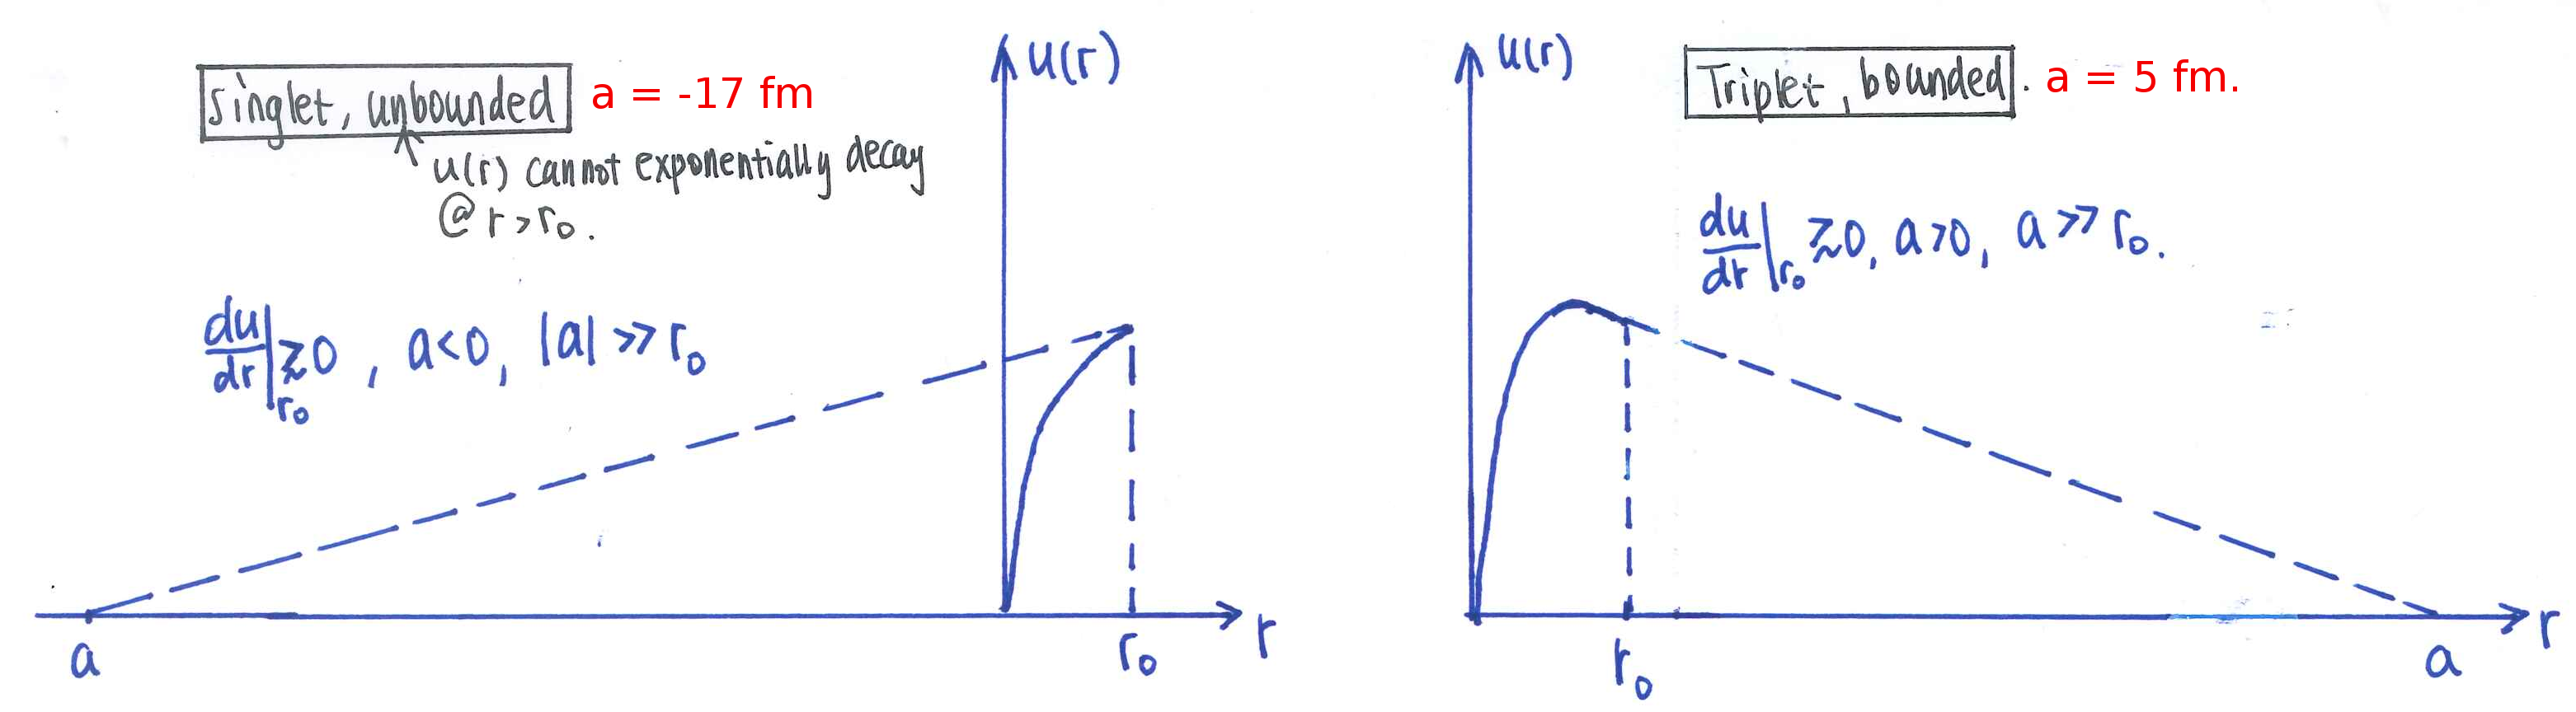
\includegraphics[width=7in]{images/scattering/s-wave-singlet-triplet.png}
\end{figure}
%
\item Know that negative potential is attractive, pulling the wave function in, $\delta_0 >0$, vise versa (recall the graph). 
%
\item Applying S-wave to n-p scattering
\begin{align}
\sin^2 (\delta_0) &= \frac{1}{1 + \left( \frac{k_2^B}{k_2} \right)^2 } \\
\sigma &= \frac{4\pi}{k^2} \sin^2 (\delta_0) = \frac{4\pi}{k_2^2 + \left(k_2^B \right)^2 } = \frac{4\pi \hbar^2}{2 \mu (E + E_B) } \xrightarrow{E \ll E_B} \frac{4 \pi \hbar^2}{2 \mu} \frac{1}{E_B} 
\end{align}
Plug in $E_B = 2.22$ MeV, we get $\sigma = 2.3$ b, which is significantly smaller than the 20 b measured. The missing piece is the spin-spin coupling:
\begin{align}
\sigma( \theta) &= \frac{3}{4} \sigma_T (\theta) + \frac{1}{4} \sigma_S (\theta) = \frac{3}{4} \frac{1}{k_2^2} \sin^2 (\theta_{ot} ) + \frac{1}{4} \frac{1}{k_2^2} \sin^2 (\theta_{os} ) \\
\sigma &= 4 \pi \sigma (\theta) = \frac{4 \pi \hbar^2}{2 \mu} \left[ \frac{3}{4} \frac{1}{E_B} + \frac{1}{4} \frac{1}{E^*} \right] 
\end{align}
Plug in $E_B = 2.22 \fsp \MeV, E^* = 0.077 \fsp \MeV$, $\sigma = 19$ b, which is a good approximation for 20b.
%
%
\item In nuclear interaction section, we talked about:
    \begin{align}
    \cos \theta &= \frac{1+ A \cos \theta_C}{\sqrt{A^2 + 1 + 2A \cos \theta_C} } \\
    \frac{E^{\prime}}{E} &= \frac{A^2 + 2A \cos \theta_C + 1}{(A+1)^2} \\
    \expect{ \frac{E^{\prime}}{E} } &= \frac{(A-1)^2}{(A+1)^2} = \alpha 
    \end{align}
    know $P(\mu)$ graph, know $P(E \to E^{\prime})$ graph.
\end{enumerate}


\end{document}

